\section{introduction}
\label{eq:sec_introduction}

%Layout the major questions. Then address the answers. Finally, construct the logical flow of necessary statements. Each sentance should be defendable and contain well defined or cited jargon. 

% \section{these are the questions I want to address}
% 
% \begin{itemize}
%  \item What field am I in?
%  \item Thesis statement: develop a criterion for AL/diffusion transition in active random media
%  \item Historically speaking, how did we get here?
%  \item When does AL versus diffusion occur?
%  \item What currently exist for criteria?
%  \item How are those criteria modeled numerically?
%  \item How do I plan on accomplishing the result desired in the thesis statement?
% \end{itemize}

%\subsection{What field am I in?}
%In solid state physics and optics, transport measures how much of something reaches the other side, and by what mechanism. 

\subsection{mesoscopic light transport}
\label{sec:what_field_am_i_in}
In this dissertation, a study of the propagation of light waves in media with randomly placed scatterers is made. Interest in the effect of self-interference of waves on transport in mesoscopic-scale media applies to fundamental questions of conductivity
\cite{1988_Stone}\cite{1997_Imry}
and has spurred new investigations of light\cite{2009_Mendez}\cite{2008_Stone}\cite{1990_Sheng}.
The mesoscopic length scale is defined as being large enough that atomic scattering mechanisms are ignored but small enough so that quantum wave effects such as phase coherence are present \cite{2005_Duan_Guojun}. %page 251 
The mesoscopic scale is important because the coherence length, over which the phase of the wave is not altered, is longer than the longest dimension of a medium, system length~$L$ (c.f. Table~\ref{tabl:lengths}). %(the difference between starting and end location for transport). 
At this scale, the effect of many scatterers is studied with respect to transition from diffusive behavior, where transmission~$T \propto \ell_{tmfp}/L$, to Anderson Localization\cite{1958_Anderson}\cite{2009_Lagendijk_PT}~(AL), where~$T \propto e^{\frac{-L}{\xi}}$. 
%Historically speaking, how did we get here?
Although AL was initially developed in the context of self-interference of de~Broglie waves and electrons\cite{1985_Lee}\cite{2008_Evers_Mirlin_rmp}, the concept applies to any wave phenomenon, including light waves\cite{1984_John_prl}.
% The relation between unitless conductance and transmission is $g=T=\sum_{ab} |t_{ab}|^2$ \cite{1998_Brouwer}
 Both AL and diffusion are defined in passive (which implies conservation of number of particles) media of infinite length, but experiments %usually 
take place in finite\cite{1979_Anderson} active media, where the number of photons changes due to gain or absorption. %[ties to thesis statement]
  
\subsection{The need for a Criterion for localization transition in active media}
\label{sec:thesis_statement}
The purpose of this dissertation will be to develop a criterion for the AL/diffusion transition in active random media. 
% HOW?
To study the transition, numerical simulations of wave guides, described in \S \ref{sec:method_numerical}, are used.
% WHY?
%P. W. Anderson said, ``one has to resort to the indignity of numerical simulations to settle even the simplest questions about it.'' \cite{1977_Anderson_nobel} 
% I want to make the distinction why diffusion can be analyzed analytically, whereas AL cannot.
The reason the AL/diffusion transition resists analytical treatment is because the approximations for diffusion are made based on the assumption that the wavelength~$\lambda$ is much less than distance between scattering events, whereas AL occurs when the direction of propagation is randomized (over transport mean free path~$\ell_{tmfp}$) on the scale of a single wavelength. That is, the diffusion process is valid for $k \ell_{tmfp} >> 1$ (with $k=2 \pi/\lambda$), whereas AL occurs when $k \ell_{tmfp} \approx 1$\cite{1960_Ioffe_criterion}. Thus, AL can not use the same approximations as diffusion.
Although this work focuses on the transition process in the context of light, results apply to any self-interference of waves in active media, such as acoustics\cite{1985_Kirkpatrick}\cite{2006_Yamilov_Weaver}\cite{2008_van_Tiggelen_Nature}.
%astronomy: the book 'Radiative transfer' by Chandrasekhar does not contain the phrase AL
%seismic waves: the book 'Quantitative seismology' by Keiiti Aki, Paul G. Richards does not contain the phrase anderson localization
 One application of this criterion would be to determine when lasing in experiments with active random media \cite{1999_Cao_RandomLaserPRL}\cite{2005_Cao} is due to strong localization rather than diffusive random lasing\cite{2008_Wiersma}.

To determine whether AL or diffusion (or neither) is affecting transport of light, three regimes are defined for quasi-one dimensional (quasi-1D) waveguides. When few scattering events occur in transmission, the ballistic regime is characterized by the average distance between scatterers (scattering length $\ell_{scat}$). If a wave encounters a sufficient number of scatterers such that the original direction is randomized (transport mean free path $\ell_{tmfp}$), then diffusion is occurring. Finally, the localized regime is encountered when scattering is sufficient such that coherent self-interference of waves stops diffusion (characterized by localization length $\xi$). Which of these three transport regimes a passive quasi-1D experiment is in can be determined by a single parameter, such as unitless conductance\footnote{Conductance $G=\frac{e^2}{h}Tr(tt^+)=\frac{e^2}{h}g$\cite{1981_Abrahams}} $g$ \cite{1979_Anderson}:  $g>1$ signifies diffusion, whereas $g<1$ indicates AL. The term ``parameter'' refers to an observable which varies in correlation to change in transport phenomena. For passive media, single parameter scaling finds that any parameter can determine the applicable transport regime as long as it has one-to-one correspondence with unitless conductance~$g$. The photonic and electronic systems are related by transmission and conductance\cite{1981_Fisher}:
\begin{equation}
 T = \sum_{a,b} |t_{ab}|^2 = g
\end{equation}
where $T$ is the total transmission flux (percentage of incident flux transmitted), and $t_{ab}$ is a complex number describing the amplitude and phase for each incident channel $a$ and output $b$. For electronic systems $g$ is measured, whereas in photonic systems one can also measure, in addition to $T$, incident-channel resolved transmission $T_{a}$ and speckle $T_{ab}$. 
\begin{equation}
\begin{gathered}
 T_a = \sum_b |t_{ab}|^2 \\
 T_{ab} = |t_{ab}|^2
\end{gathered}
\end{equation}

Active media is an exception to single parameter scaling because it is non-conservative and thus breaks the one-to-one correspondence\cite{1994_Freilikher_absorption}. Although measurement of transmission yields a value, it does not correspond to a specific transport regime. $T>1$ may be due to the presence of gain in localized media, and $T<1$ may be due to absorption present in media in the diffusive regime. Thus a two parameter space is required to describe the AL/diffusion transition in active media: how active the medium is, and what transport regime the equivalent passive system would be in. A criterion is needed to characterize when an experiment is in a specific regime in order to recognize what phenomena affects transport.

\subsection{passive criteria currently available}
\label{sec:passive_criteria}
Currently, there exists AL/diffusion transition criteria for passive media. 
% motivation for alternatives to $g$?
% Ioffe-Regel \cite{1960_Ioffe_criterion}: the AL/diffusion transition is $ k \ell_{tmfp} \approx 1$.
For example, Thouless \cite{1977_Thouless} showed that whether the peaks in density of state are distinguishable or not over a range of frequencies demonstrates the transition. The ratio of average widths of the density of states (DOS) $\delta \omega$ to peak-to-peak separation $\Delta \omega$ returns a unitless number indicating whether the experiment is affected by AL or diffusion. 
\begin{equation}
\frac{\delta \omega}{\Delta \omega} \propto g
\label{eq:Thouless_passive}
\end{equation}
When peaks are distinguishable, then AL is occurring and $g<1$. However, this is not a valid criterion in active media because gain also decreases mode width.

Another approach is to recall that the transition from diffusion to AL implies a cessation of the diffusion description and assumptions of the standard diffusion equation are invalid. In an effort to extend the applicability of the diffusion equation, self-consistent theory of AL \cite{1980_Vollhardt_Wolfle}\cite{2008_Cherroret} was developed. Without self-interference of waves, the diffusion coefficient $D_0$ is constant throughout the medium. However, when the path of a wave crosses itself and can self-interfere, the diffusion coefficient decreases.
%why?! if both constructive and destructive interference are accounted for, it is not obvious that one or the other should dominate 
Since path loops can not form near the boundary of a sample, the diffusion coefficient becomes position dependent $D(z)$. Thus, the change from constant~$D_0$ to position-dependent $D(z)$ signifies the transition to AL. However, this extension does not describe full Anderson localization.

There are many other criteria, including correlation functions \cite{2005_Yamilov_correlations}\cite{1999_van_Tiggelen}of observables and the inverse participation ratio $\langle {\cal E} \rangle^2 / \langle {\cal E}^2 \rangle$ for energy in the medium ${\cal E}$. One motivation for the diversity of criteria is the desire for easy experimental measurement. The search for better criteria is possible because single parameter scaling means all are equivalent in passive media. More recently, there is an effort to find a criterion for active photonic random media; for example, a ratio developed in the context of an experiment with microwaves in waveguides with disordered absorbing media\cite{2000_chabanov_nature}: $var(T/\langle T \rangle)$. However, the ratio $T/\langle T \rangle$ may not be useful in media with gain since $\langle T \rangle$ is not well defined (given a sufficiently large number of random media with some gain, a few will lase) and $T$ diverges as gain is increased. Conditional statistics are used in this dissertation to avoid the first issue. %In numerical simulation, gain and absorption are easily adjusted.

\subsection{$T/{\cal E}$ as a candidate for diffusion-localization transition criterion}
\label{sec:te_ratio_candidate}

In media with gain, transmission $T$ of light theoretically diverges as random lasing threshold (RLT) is approached (since a saturation mechanism is model specific). To eliminate the divergence, normalize $T$ by the energy in the medium ${\cal E}$. Although both quantities diverge at RLT, it can be shown from the diffusion equation in active media\cite{2009_Payne_TE} and by conservation of energy that the ratio $T/{\cal E}$ approaches a constant. Start from conservation of energy (${\cal E} =\int_0^L{\cal W}(z)dz$) with respect to flux $J$,
\begin{equation}
\frac{\partial {\cal W}}{\partial t} + \vec{\nabla} \cdot \vec{J} = \frac{{\cal W} c}{\ell_g} + J_0 \delta(z-z_p)
\label{eq:conservation_flux}
\end{equation}
where $z_p$ is penetration depth, $\ell_g$ is gain length, and $c$ is speed of light. Assuming steady state in 1D, 
\begin{equation}
\frac{d J_z}{dz} = \frac{{\cal W} c}{\ell_g} + J_0 \delta(z-z_p)
\label{eq:oned_no_time_JW}
\end{equation}
integrate both sides with respect to $z$ over the length of the medium to get the equation for conservation of energy for an active medium
\begin{equation}
T + R -1 = {\cal E} \frac{c}{\ell_g J_0}
\label{eq:conservation_energy_active_medium}
\end{equation}
In the limit that gain length $\ell_g$ approaches RLT (critical gain length $\ell_{g_{cr}}$), both $T$ and $R$ go to infinity. Assuming $T \approx R$,
\begin{equation}
\frac{T}{{\cal E}} = \frac{c}{2 \ell_{g_{cr}}J_0}
\label{eq:TE_RLT_limit}
\end{equation}
This constant is disorder-specific due to $\ell_{g_{cr}}$, so $T/{\cal E}$ must be found before averaging or higher moments.

For gain below RLT, by comparing the measured $T/{\cal E}$ in an experiment to the $T/{\cal E}$ found from a diffusion-based prediction, the deviation would be due to wave interference effects (and thus constitute a signature of AL). For passive media, deviation from the diffusion prediction for $T/{\cal E}$ is equal\cite{2009_Payne_TE} to the well-established \cite{2008_Cherroret} $D(z)$ from self-consistent theory of AL (see Appendix~\ref{sec:appendix_TE_Dz_relation}).
\begin{equation}
T/{\cal E} \approx \frac{1}{J_0} \frac{2 D_0}{L^2} \left(\frac{1}{L} \int_0^L \frac{D_0}{D(z)} dz \right)^{-1}
\label{eq:TE_related_Dz}
\end{equation}
Since $T/{\cal E}$ is equivalent to $D(z)$, then experimentally $T/{\cal E}$ should behave as $D(z)$ does with respect to $D_0$ for passive media: decrease as self-interference of waves increases. Therefore, it appears that $T/{\cal E}$ is a good criterion for AL/diffusion transition in active media since it is measurable, does not diverge in active media, and is related to an established passive criterion $D(z)$.


\subsection{Method of study of criteria for diffusion-localization transition}
\label{sec:method_numerical}
%\subsection{What methods are used by others?}
When P. W. Anderson initiated the field of localization due to self-interference of waves, he did so using a new model for solid state transport, the Anderson tight-binding Hamiltonian\cite{1958_Anderson}, which applies to arbitrary medium size and dimension. For quasi-1D geometry, Random Matrix Theory (RMT)\cite{1951_Wigner} % origin
\cite{1997_Beenakker} % review, 
%uses the fact that the total transfer matrix is unitary, but the elements of that matrix are assumed to be random.
%%% get citations from page 103 of Vellekoop's thesis
%Then the effect on various parameters is observed when a few more scatterers are added to the medium using transfer matrices (perturbing the length of the waveguide).  
is widely used. However, neither of these approaches are able to describe the electric field (and thus total energy ${\cal E}$) inside a random medium.

%How will I accomplish the result desired in the thesis statement?
To study AL criteria for random media, two numerical models have been developed. The first is a one dimensional (1D) set of layers of alternating-valued dielectric material with random widths. This model was developed to find transmission ($T$) and energy inside the medium (${\cal E}$) as a possible criterion $T/{\cal E}$ for active media\cite{2009_Payne_TE} \cite{2009_Payne_loc_criterion}. It was verified that the ratio $T/{\cal E}$ is not divergent, even as lasing threshold is approached (as expected). The 1D system was used because AL is known to occur and diffusion can not happen, thus observed effects were not due to diffusion.
% based on work of slab with active media in diffusive regime
% T/E related to D(z)
% (T_g/E_g)E_p reduces to g in passive media
Since diffusion is not possible in 1D systems, a planar quasi-1D metallic waveguide model with randomly-placed scatterers was developed to study the simplest AL-diffusion transition and to investigate the other listed criteria ($D(z)$, inverse participation ratio, $T/{\cal E}$).  This model is needed since, even for passive systems, no plot of $D(z)$ in the diffusive regime and based on Maxwell's equations (c.f. Fig.~\ref{fig:Dz_passive}) is available in the literature.

\begin{figure}
\vskip -0.5cm
\centerline{
\scalebox{.5}{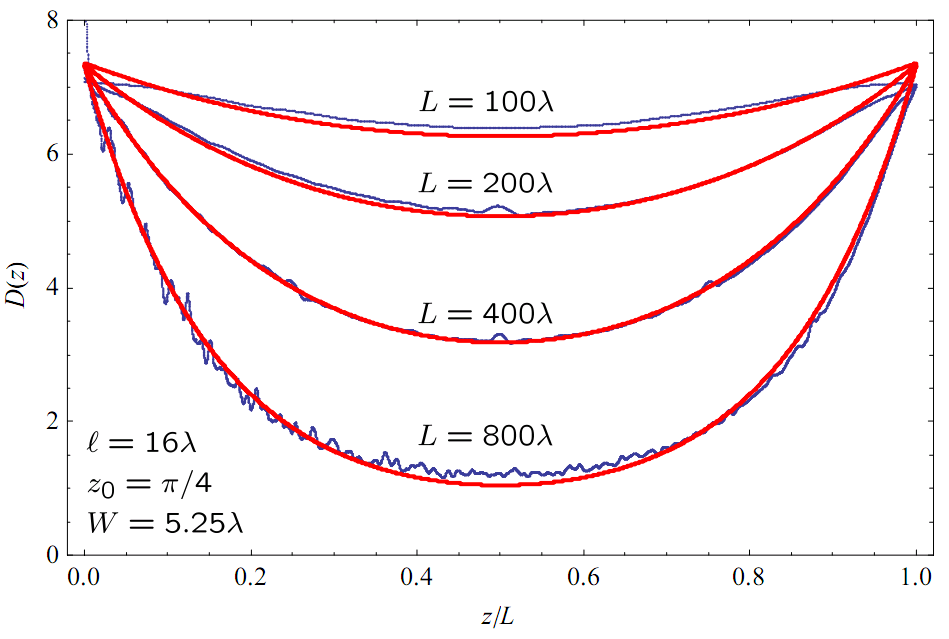
\includegraphics{pictures/Dz_passive}}}
\vskip -0.5cm
% NOTE: if a short caption is needed for figure list, use
%\caption[short desk]{long desk}
\caption{Position dependent diffusion coefficient $D(z)$ as predicted by self-consistent theory of localization (smooth red curves) and numeric results (rough blue lines) for quasi-1D waveguides with randomly-placed passive scattering potentials for varying system length $L$, constant scatterer density and width $W$. Very good agreement for ballistic ($L=100 \lambda$), diffusive, and localized ($L=800 \lambda$) regimes. $\ell$ is transport mean free path and $z_0$ is penetration depth.}
\label{fig:Dz_passive}
\end{figure}

%Method: How am I numerically modeling these criteria?}
To develop numerical models that can simulate wave transport in active media for individual realizations of disorder, the transfer matrix method \cite{1981_MacKinnon_scaling}
% note: when MacKinnon cites tmm, he uses 1981_MacKinnon_scaling and 
% MacKinnon A 1994 J. Phys. Condensed Matter 6, 2511
\cite{1992_Pendry}\cite{2003_Kettemann} is implemented for the entire quasi-1D waveguide. Essentially, the transfer matrix method matches boundary conditions before and after an event in a system where wave modes are quantized. The quasi-1D geometry is not only experimentally viable \cite{2009_Genack_PRB}, it also provides a convenient theoretical framework\cite{1982_Dorokhov_DMPK}\cite{1988_Mello_Kumar_DMPK}. Quasi-1D geometry has the following characteristics in this dissertation: (1)~quantized transverse modes due to boundary conditions ($E(y=0,W;\forall z)=0$ as for metallic edges), (2)~waveguide width $W < \ell_{tmfp}$ such that no significant transverse propagation occurs, and (3)~aspect ratio ($L:W$) is not fixed: $W$ is constant when $L$ is increased (with fixed scatterer density). Further, the geometry is restricted to two dimensions in order to study a single polarization.

For light waves, transverse wave quantization means modes of electric field and its derivative can be written in the form of a vector. The translation of that field in vector form through a dielectric-filled space or past a scattering potential is described by a matrix, the rank of which is dependent on the number of transverse modes of the waveguide (c.f. Appendix~\ref{sec:appendix_derivation_transfer_matrices_quasi1d}).
\begin{equation}
 \left( \begin{array}{cc}
T_{11} & T_{12} \\
T_{21} & T_{22} \\
\end{array} \right)
\left( \begin{array}{c}
E_0 \\
E_0^{\prime}
\end{array} \right)
=
\left( \begin{array}{c}
E_{\Delta x} \\
E_{\Delta x}^{\prime}
\end{array} \right)
\end{equation}
Many of these matrices multiplied together represents multiple scattering events: $\hat{T}_{total} = \prod_i \hat{T}_i$. The product of these matrices describes the effect of the medium on transport of the incident light. The derivation of the transfer matrix method is \textit{ab initio} based on Maxwell's equations\cite{1999_Jackson} and no assumption about transport mean free path is made. As shown in Appendix~\ref{sec:appendix_derivation_transfer_matrices_quasi1d}, the differential wave equation
\begin{equation}
\nabla^2 E(\vec{r}) = - \frac{\omega^2}{c^2} E(\vec{r})
\label{eq:wave_equation_electric_field_introduction}
\end{equation}
can be separated into perpendicular and parallel components (resolving wave vector $\vec{k}$ into $k_{\perp}$ and $k_{\parallel}$). Once the electric field solution is found, scattering potentials are introduced, initially as $\delta$ functions. Since the transfer matrices have finite rank, the scattering potentials used are actually a finite summation of Fourier components of the $\delta$ function. Although the purpose of the numerical model is a study of the passive criteria in active media, the resulting electric field magnitude, plotted in Fig.~\ref{fig:electric_field_zoomed}, is a secondary benefit of using this model.

\begin{figure}
\vskip -0.5cm
\centerline{
\scalebox{.5}{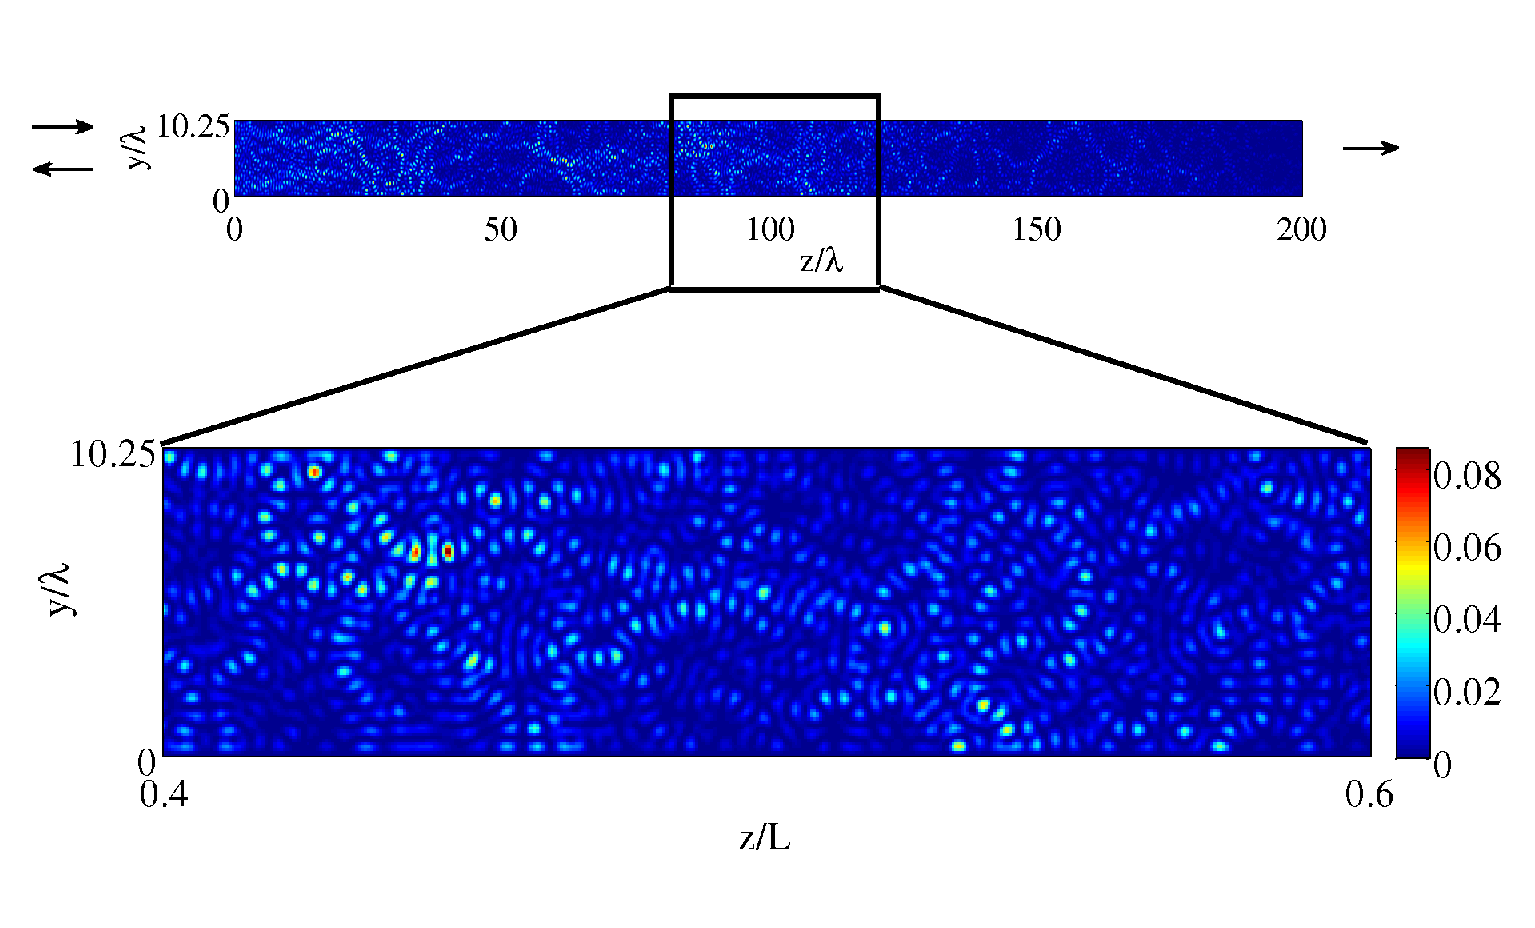
\includegraphics{pictures/electric_field_resonant_freq_zoom_normalized_z_box_arrows}}}
\vskip -0.5cm
% NOTE: if a short caption is needed for figure list, use
%\caption[short desk]{long desk}
\caption{Magnitude of electric field inside a quasi-1D waveguide for passive media in the diffusive regime. Mid-section of waveguide is shown (from $z/L=80/200$ to $z=120/200$) for a resonant frequency (higher than average transmission). Spatially varying field intensity (with continuous wave incident flux) demonstrates interesting microscopic behavior, even though the system is in the diffusive regime.}
% The Poynting vector can plotted
% [don't say this because you aren't including a picture of the Poynting vectors.]
\label{fig:electric_field_zoomed}
\end{figure}

The transfer matrix method is in use by others\cite{2007_Froufe-Perez_PRE}, but its application is usually limited to either Random Matrix Theory for perturbitive study or directly only in the diffusive regime. This is due to the fact that multiplication of numerical matrices results in inaccuracy due to divergent eigenvalues\cite{1968_Osedelec}.
% A simple showing of this would be nice
The numerical inaccuracy is detectable since each transfer matrix has determinant unity (due to conservation of flux). 
% determinant is the scaling factor by which volume changes. Is that why the det(A)=1? Flux conservation?
It can be shown that the product of the matrices must retain a determinant of unity since
%citation would be nice here, but most linear algebra books leave it as an excersise to the reader
\begin{equation}
det(\hat{A})det(\hat{B})=det(\hat{A}\hat{B})
\end{equation}
To renormalize the divergent eigenvalues and make this approach feasible, self-embedding technique \cite{2001_Yamilov} \cite{1999_yamilov_selfembed}  \cite{1976_Bellman_Wing_embedding} is applied.
%
% How it works mathematically
%
Although self-embedding technique applies to any numerical multiplication of many matrices, it is applied here to waveguides.%1D and planar quasi-1D waveguide geometries.
The reliability of the transfer matrix method with self-embedding is demonstrated by comparing numerical simulation results of average unitless conductance $\langle g \rangle$ versus variance $var(g)$ to data found from a supersymmetry approach (theoretical)\cite{2000_Mirlin}. With no fitting parameters, there is very good agreement (c.f. Fig.~\ref{fig:Mirlin_supersymmetry_g_varg}). Similarly, the diffusion coefficient from numerical simulation of passive media matches expected $D(z)$.

\begin{figure}
\vskip -0.5cm
\centerline{
\scalebox{.45}{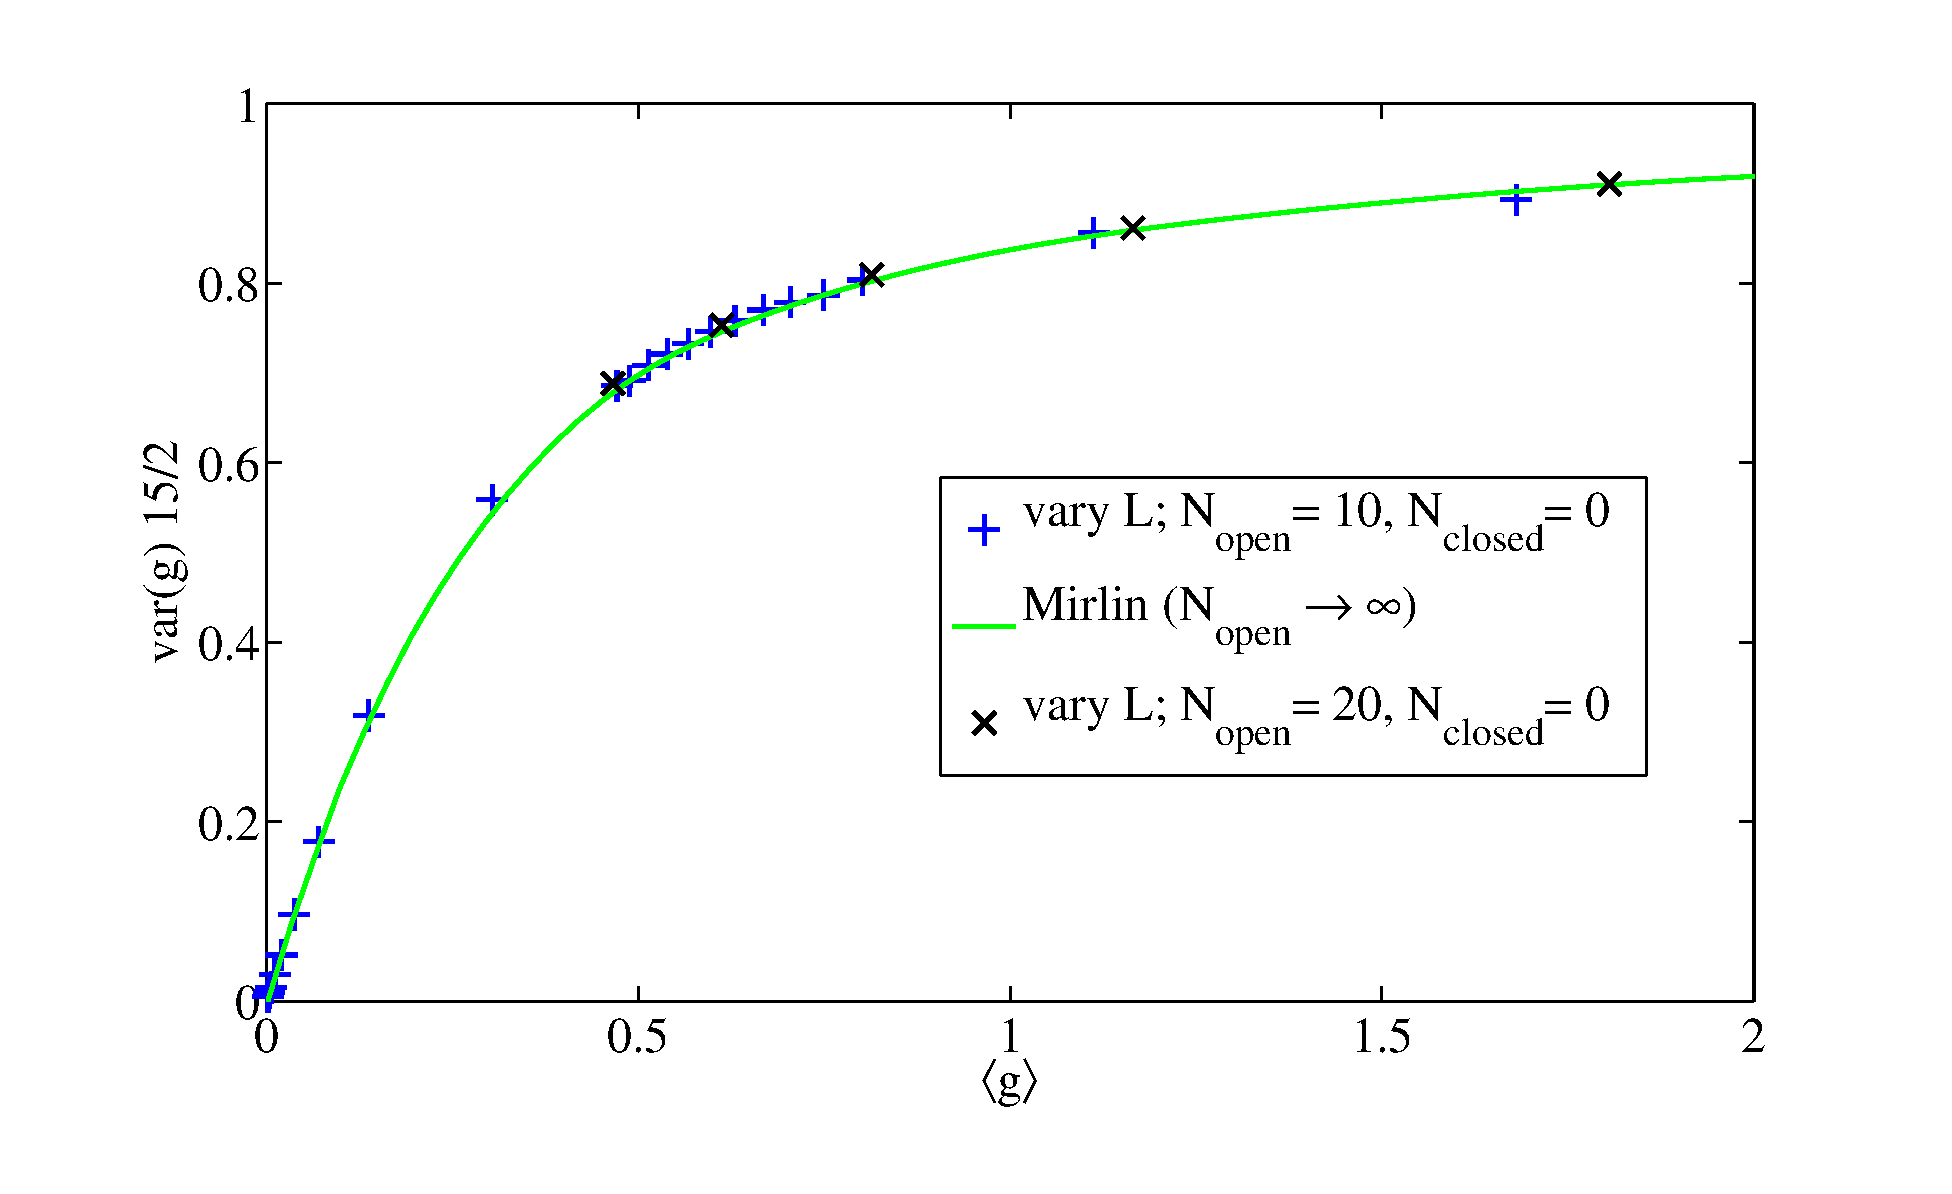
\includegraphics{pictures/var_g_versus_g_no_closed_channels}}}
\vskip -0.5cm
% NOTE: if a short caption is needed for figure list, use
%\caption[short desk]{long desk}
\caption{Theoretical prediction from supersymmetric approach for average unitless conductance $g$ versus variance of $g$ for quasi-1D waveguide\cite{2000_Mirlin} compared to results from numerical simulations described in \S \ref{sec:method_numerical}. No fitting parameters are used and good agreement is found. The $15/2$ accounts for the geometry of the waveguide. $\langle g \rangle$ and $var(g)$ for waveguides of two different widths (number of open channels $N_{open}$ is determined by $W$) and varying system length $L$ were found from many realization of random media for each waveguide geometry. The supersymmetry-based approach assumes the limit of an infinite number of propagating modes, but $N_{open}=10$ and $20$ is sufficient.}
\label{fig:Mirlin_supersymmetry_g_varg}
\end{figure}
  

\subsection{Outline of transport regimes}
\label{sec:twod_plot}
To guide the study of the extension of the three passive regimes in active media, a two parameter diagram (c.f.~Fig.~\ref{fig:regime_plot_main}) was developed to enumerate types of transport behavior. The two-parameter plot is needed in order to define specific signatures of diffusion and AL in active media. The chapters that follow will use the numerical model of the quasi-1D waveguide to verify transitions between types of transport and to characterize behavior of passive-based criteria and the proposed $T/{\cal E}$ in active random media.

A single-valued parameter such as $T/{\cal E}$ is useful even in this two-parameter space since it only characterizes whether diffusion or AL is affecting transport. However, not all single-valued criteria are applicable due to the divergence of most observable parameters as RLT is approached with increased gain. Before a determination of which side of diffusion or AL $T/{\cal E}$ characterizes, the behavior on both sides must be defined. Currently, no clear definitions of AL or diffusive behavior exist for active random media.

%\subsection{what is the plan?}
Fig.~\ref{fig:regime_plot_main} describes types of transport in quasi-1D waveguides with randomly-placed scatterers and has three passive regimes (\textbf{B}allistic, \textbf{D}iffusive, \textbf{L}ocalized) on the horizontal axis and \textbf{G}ain or \textbf{A}bsorption on the vertical axis. The two letter combinations on the plot denote a regime of specific behavior. The passive regime transitions (B/D/L) are characterized by transport mean free path $\ell_{tmfp}$ and localization length $\xi$, as described in \S \ref{sec:thesis_statement}. All lengths are normalized by wavelength $\lambda$. 

\begin{figure}
\vskip -0.5cm
\centerline{
\scalebox{.75}{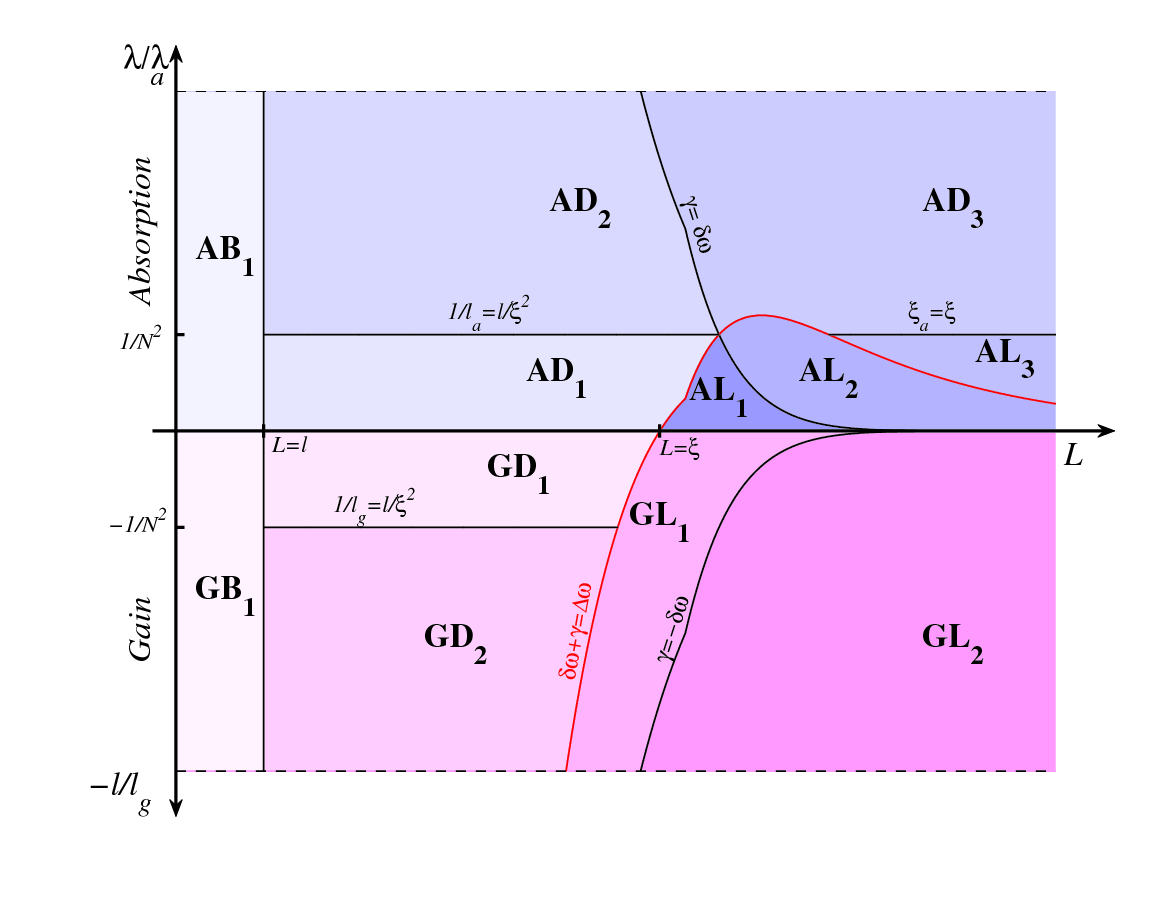
\includegraphics{pictures/regimes_plot_main}}}
\vskip -0.5cm
\caption{Passive transport regimes on the horizontal axis, strength of active media plotted vertically. Various types of transport phenomena denoted by two letter abbreviations (see text for explanation). Each region is a permutation of the inequality of relevant characteristic lengths.
%Regime plot for quasi-1D random media. Lines denote transitions between regions of similar transport behavior; each region is denoted by a two-letter abbreviation. See text for explanation.
}
\label{fig:regime_plot_main}
\end{figure}

%It is important to note that characteristic lengths are defined in specific regimes. For example, 
%For brevity, only absorption is referred to, but the concepts apply equivalently to gain. 
The absorption (gain) rate $\gamma_{a,g}$ is the average number of absorption events per unit time, where an event refers to the particle removed (doubled) along a specific path. The absorption (gain) rate is the inverse of the absorption (gain) lifetime,
\begin{equation}
\gamma_{a,g} = \frac{1}{\tau_{a,g}}
\end{equation}
where $\tau_{a,g}$ is the average time the particle has before being absorbed (doubled). The ``averaging'' is over many random particle paths. Given a characteristic time $\tau_{a,g}$, a characteristic length is 
\begin{equation}
\ell_{a,g} = \tau_{a,g} c
\end{equation}
where $c$ is the propagation speed of the particle. This characteristic length is the average distance prior to absorption (doubling) with respect to the path length. The $\ell_{a,g}$ is found from the time-dependent diffusion equation in one dimension,
\begin{equation}
D \frac{\partial^2 I}{\partial z^2} = \frac{\partial I}{\partial t}
\label{eq:diffusion_equation_1D}
\end{equation}
to be 
% see /svn/bens/lab_notebook/20090422_dr_Yamilov_mtg_regime_change_for_plot.pdf
% equation 37
\begin{equation}
\ell_{a,g}= \left( \frac{d}{\pi^2}\right) \frac{L^2}{\ell_{tmfp}}
\label{eq:ballistic_gain_abs}
\end{equation}
However, $\ell_{a,g}$ is already defined in the ballistic regime as the average length after which the particle is no longer present in a ballistic system. The parameter $L$ (how far the particle would have gone along a ballistic path) should be replaced by a new diffusive-regime length, $\xi_{a,g}$. Solving Eq.~\ref{eq:ballistic_gain_abs} for $\xi_{a,g}$,
\begin{equation}
 \xi_{a,g} = \sqrt{\frac{\ell_{a,g} \ell_{tmfp}}{d}}
\label{eq:diffusive_absorption_length}
\end{equation}
Physically, $\xi_{a,g}$ is the average length after which the particle is no longer present in a multiple scattering system. To distinguish the two absorption (gain) lengths, $\xi_a$ is measured with respect to system length $L$ (rather than path length $L_D$), thus $\xi_{a,g}$ is less than $L$ in systems with absorption, whereas $\ell_{a,g}$ is measured with respect to path length $L_D$ since it is a ballistic-system length. If $L=L_D$, then no diffusion is occurring and $\ell_{a,g} = \xi_{a,g}$.  This distinction of measuring an absorption length with respect to diffusive path $L_D$ or system length $L$ is usually not made in literature for two reasons: experimentally, $L_D$ is harder to measure than $L$, second, it is usually not specified which regimes various lengths apply to.

For localized systems, it no longer makes sense to measure lengths with respect to path length since wave effects are dominant (ray optics do not apply). $\xi_{a,g}$ is used, but it is not defined in terms of $\ell_{a,g}$ as in Eq.~\ref{eq:diffusive_absorption_length}.  The transition denoting whether absorption affects AL is set by $\xi_{a} = \xi$ (horizontal line between $AD_3$ and $AL_3$ in Fig.~\ref{fig:regime_plot_main}). This transition in the diffusive regime is found by applying Eq.~\ref{eq:diffusive_absorption_length} to $\xi_{a,g} = \xi = N_{open} \ell_{tmfp}$ and solving 
\begin{equation}
N_{open}^2 \ell_{tmfp}^2 = \frac{\ell_{tmfp}\ell_{a,g}}{d}
\end{equation}
to get $\ell_{a,g} =d N_{open}^2 \ell_{tmfp}$. This line denotes for the diffusive regime how active the media must be to affect transport behavior and applies to both absorption and gain. The remaining curves in Fig.~\ref{fig:regime_plot_main}are derived from density of state transitions, rather than characteristic lengths.

The mode width $\delta \omega$ of the Thouless criterion (Eq.~\ref{eq:Thouless_passive}) is inversely proportional to the escape life time (the average time until an input leaves the system) for passive media. To account for absorption or gain, an additional term is needed in the form of a rate
\begin{equation}
\delta \omega +\gamma_{a,g}
\end{equation}
Although the density of states $\Delta \omega$ also changes as a function of gain due to Kramers-Kronig relation\cite{1999_Jackson}, the perturbation is ignored since the amount of gain and absorption of interest is small. 
% boundaries
The Thouless criterion is thus adapted to active media by inclusion of the gain or absorption rate $\gamma_{a,g}=\mp~c/\ell_{a,g}$ (gain is sometimes referred to as negative absorption\cite{1968_Letokhov}),
\begin{equation}
\frac{\delta \omega +\gamma_{a,g}}{\Delta \omega} = \delta'
\label{eq:generalized_thouless}
\end{equation}
and is plotted as the red curve $\delta'=1$. Physically, this boundary signifies whether peaks in density of state are distinguishable or not (a ratio of mode width to mode separation). Additionally, active media introduces the transition from mode width being determined by leakage to gain or absorption, as plotted by the black curve $\pm \gamma = \delta \omega$. %The remaining boundaries are straight lines and are determined by enumerating permutations of characteristic length scale inequalities. For example, in the diffusive regime, $L$, $\xi$, $\ell_{tmfp}$, and $\ell_{a,g}$ form a minimum basis for distinguishing transport behavior. 
%Enumerating all permutations of relevant length inequalities, a distinct set of transport behaviors has been found.
% caveat
Although each region is separated by a line in Fig.~\ref{fig:regime_plot_main}, the transition between regimes is actually continuous due to using many realizations of randomly placed scatterers. Given the boundaries between each region of unique transport behavior, the two letter abbreviations are defined.

% transport behavior of each regime
In the ballistic regime $GB_1$, gain (absorption $AB_1$) is not expected to change transport behavior for gain below ballistic lasing threshold (absorption length $\ell_a < L$). For a small amount of gain, $GD_1$ (absorption $AD_1$), the diffusive transport is also expected to remain similar to passive media (the use of conditional statistics\cite{2005_Yamilov_correlations} eliminates a small number of lasing media). With sufficient absorption, signatures of diffusion are reduced ($AD_2$) and suppressed ($AD_3$). In contrast, gain enhances fluctuations ($GL_1$) and leads to, on average for many realization, lasing ($GL_2$)\cite{1968_Letokhov}. Transport in $GD_2$ is the equivalent of ``negative absorption'' in $AD_2$. The remaining absorption regimes transition from distinct spectral peaks and leakage due to radiation ($AL_1$) to distinct spectral peaks with absorption dominating leakage ($AL_2$) to a continuous spectrum due to absorption with weak localization ($AL_3$).

% the hump of AL_2 is not separated because?

%The kink in the curves is the transition from diffusion based equations to Mirlin's projections\cite{2000_Mirlin} in the localized regime.


% if I only have 10 minutes of the presentation, I will not have time for these regions
\begin{comment}
\begin{figure}
\vskip -0.5cm
\centerline{
\scalebox{.75}{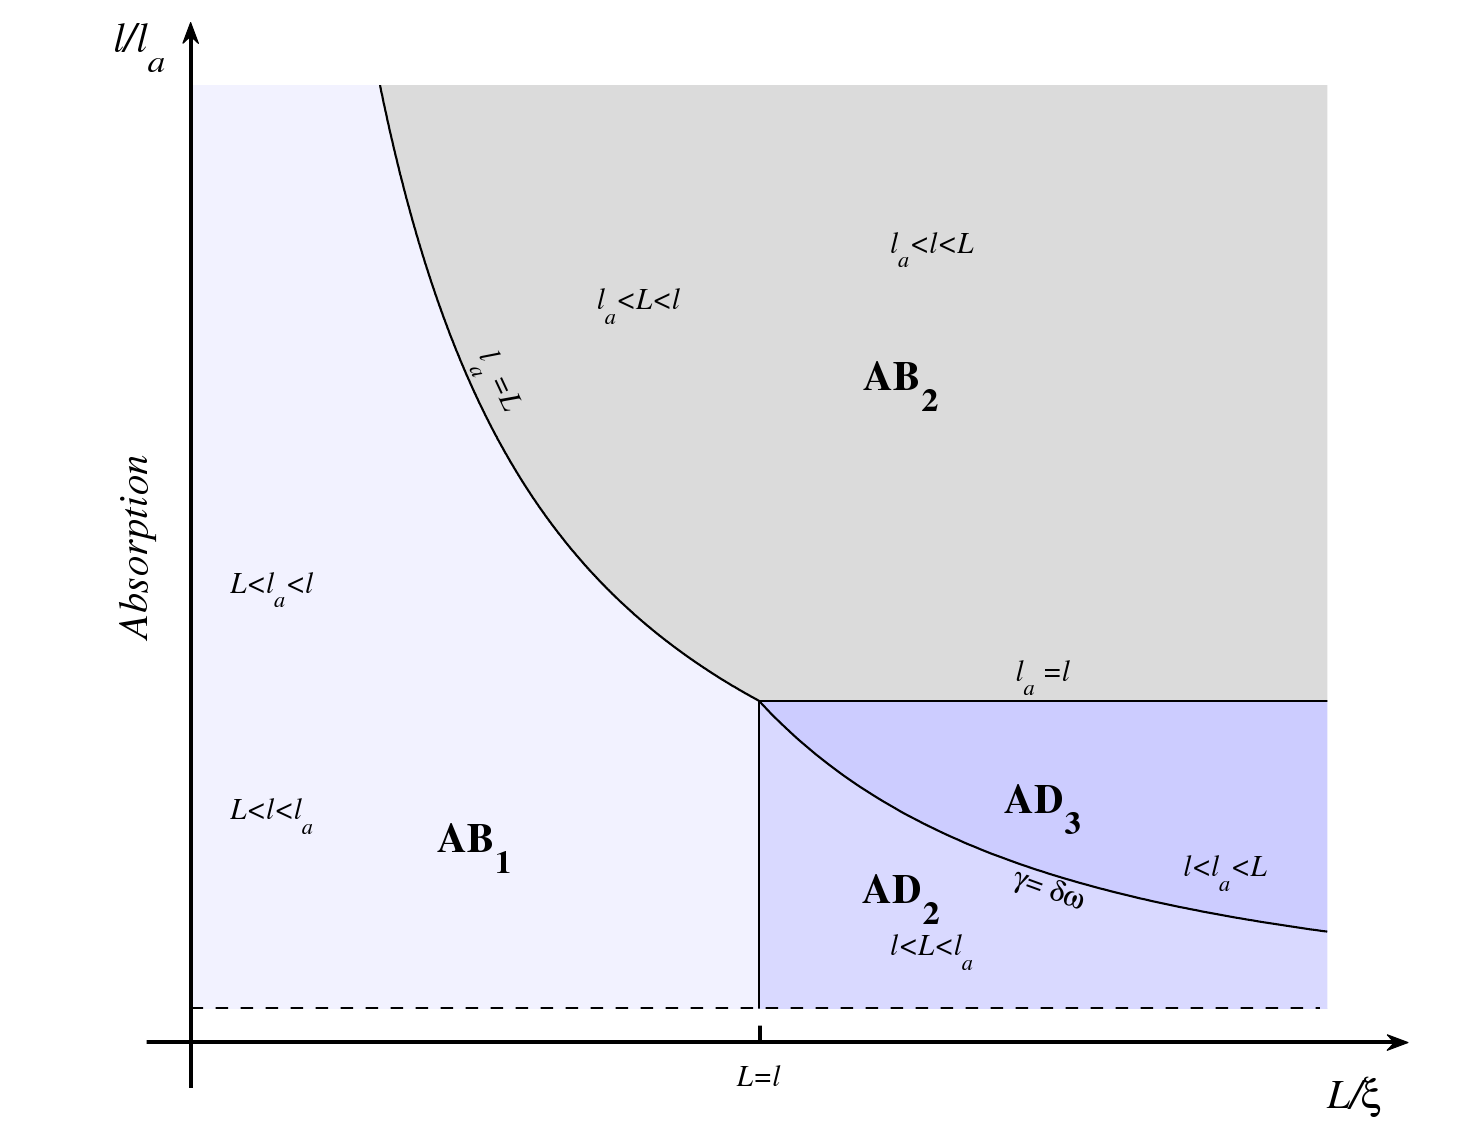
\includegraphics{pictures/regimes_plot_upper}}}
\vskip -0.5cm
\caption{
%Upper regime plot (strong absorption) for quasi-1D random media. Each region is associated with an inequality of lengths. See text for explanation.
}
\label{fig:regime_plot_upper}
\end{figure}

\begin{figure}
\vskip -0.5cm
\centerline{
\scalebox{.75}{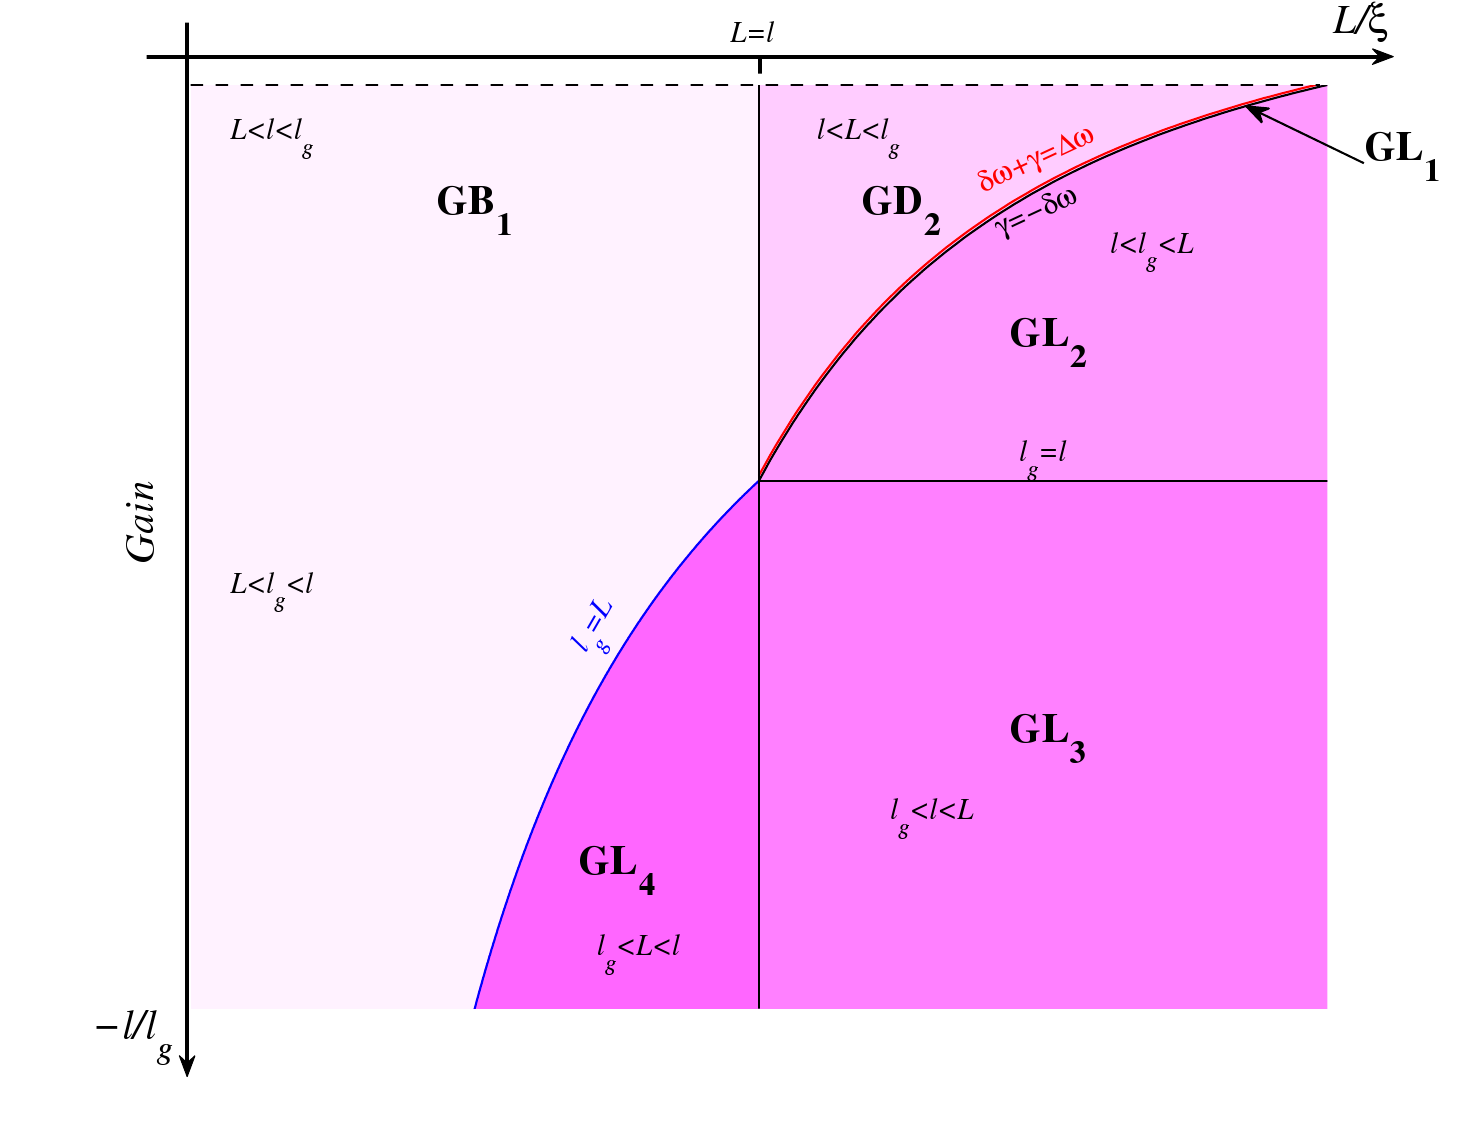
\includegraphics{pictures/regimes_plot_lower}}}
\vskip -0.5cm
\caption{
%Lower regime plot (strong gain) for quasi-1D random media. See text for explanation.
}
\label{fig:regime_plot_lower}
\end{figure}
\end{comment}

% Note: analytical quasi-1D solution found by \cite{1994_Beenakker_exact}

%I expect to be successful because I have sufficient tools (numerical model) and the plan is detailed and well-defined. Also, it is not too broad or too narrow.

To verify the boundaries and transport behaviors specified in Fig.~\ref{fig:regime_plot_main} as determined by criterion $T/{\cal E}$, the numerical model for quasi-1D waveguides with random media is used. In addition to determining the applicability of other criteria such as $D(z)$, correlation functions, and the inverse participation ratio for the active AL/diffusion transition, myriad other interesting topics are feasible with this numerical model. Examples include studying the effect of closed channels with gain\cite{2010_Payne_closed}, wave front shaping\cite{2008_Vellekoop_Mosk} to change transmission or focus field inside the medium, eigenmodes of transmission\cite{1986_Imry}, and the visualization of Poynting vector field loops. The numerical model developed serves as a robust method for a comprehensive approach to investigating the AL/diffusion transition for the quasi-1D waveguide geometry with active random media.

\newpage
% http://www.andy-roberts.net/misc/latex/latextutorial4.html
% http://en.wikibooks.org/wiki/LaTeX/Tables
\begin{center}
\begin{table} % for label and caption purposes
%\begin{tabular}{|l|l|l|}
\begin{tabular}{|l|l|p{6cm}|}
%\begin{tabular*}{0.75\textwidth}{|l|l|l|}{@{\extracolsep{\fill}} | c | c | c | }
\hline symbol & name & description \\ \hline
$\lambda$ & wavelength & Wavelength of incident light \\ 
$L$ &  system length & Length of waveguide along direction of propagation ($z$-axis) \\ 
$W$ & system width & Dimension of waveguide perpendicular to direction of propagation ($y$-axis) \\
$L_D$ & path length & How far a particle (i.e. ray optics) travels in the media in ballistic and diffusive regimes \\
$\ell_{scat}$ & scattering length & Average distance between scattering events. Often referred to as $\ell_{mfp}$ (mean free path) or the inelastic length\cite{1984_John_prl}, or extinction length\cite{1999_van_Tiggelen}. \\ 
$\ell_{tmfp}$ & transport mean free path & Average distance over which phase and direction are randomized.  $\ell_{tmfp} = \frac{\ell_{scat}}{1-\langle cos\ \theta \rangle}$. Measured with respect to $L$. \\ 
$\xi$ & localization length & Probability of diffusive path forming loop is 1.  $\xi~=~N~\ell_{tmfp}$. Measured with respect to $L$. \\ 
$\ell_{a,g}$ & ballistic absorption/gain length & Average distance over which intensity decreases by two/increases by two. \\
$\xi_{a,g}$ & absorption/gain length & How far, on average, a particle travels in the diffusive regime before being absorbed (or doubled), measured with respect to path length $L_D$ in the diffusive regime \\ 
$z_p$ & penetration depth & Applies to diffusive regime only. $z_p \approx \ell_{tmfp}$ \\ \hline
\end{tabular}
\label{tabl:lengths}
\caption{Lengths used in the dissertation. All (except $\lambda$) are normalized by wavelength.} % lengths can be converted to equivalent times by $\ell = c t$
\end{table}
\end{center}